% "Станет проще"

\documentclass[a4paper,12pt]{article} % тип документа

% report, book

% Рисунки
\usepackage{graphicx}
\usepackage{wrapfig}
\usepackage{hyperref}
\usepackage[rgb]{xcolor}
\pagestyle{plain}
\usepackage{floatflt}
\usepackage{multirow}
\usepackage{lipsum}
\usepackage{amsmath, amstext}
\usepackage{siunitx}
%\usepackage{subcaption}
\usepackage{wrapfig}
\usepackage{mathrsfs}
\usepackage{adjustbox}
\usepackage{enumerate, indentfirst, float}
\usepackage{pgffor}
\usepackage{capt-of, svg}
\usepackage{array}
\usepackage{longtable}
\usepackage{csvsimple}
\usepackage{pdfpages}
\usepackage{subfigure}
\usepackage{sectsty}



%  Русский язык

\usepackage[T2A]{fontenc}			% кодировка
\usepackage[utf8]{inputenc}			% кодировка исходного текста
\usepackage[english,russian]{babel}	% локализация и переносы



% Математика
\usepackage{amsmath,amsfonts,amssymb,amsthm,mathtools} 

\usepackage{wasysym}

%Заговолок
\author{Сафиуллин Роберт	}
\title{Эффект Талбота}





\begin{document} % начало документа

\maketitle


\newpage

\section{Цель работы:}
Экспериментальное изучение эффекта Талбота 
\\
\section{В работе используются:}
 Линза, экран, лазер, зрительная труба, набор дифракционных решеток
 
        \section{Теория}
        Рассмотрим дифракционную решетку. Для простоты будем считать ее периодичной только по одной оси. \\
        Пусть слева на экран падает плоская волна вдоль оси z: \\
\begin{center}

        A(x,z)=$A_0 e^{ikz}, z<0$  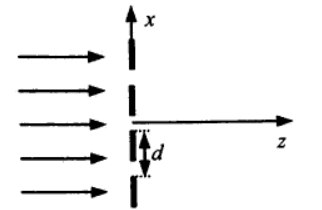
\includegraphics[scale=0.8]{ust}\\
        \end{center}        

        Вследствие периодичности структуры справа от него при z=+0 поле может быть представлено в виде ряда Фурье: \\
\begin{center}

        $A_S(x)=A(x,z)|_{z=+0}=D(x)A(x,z)|_{z=-0}=\sum a_n e^{iu_n x} $ \marginpar{(1)}\\
        \end{center}       

        , где $u_n=n\Omega, \Omega=2\pi/d $,
        d-период решетки. \\ Каждое слагаемое в сумме (1) порождает в области z>0 волну \\
        \begin{center}
        $a_n e^{iu_n + iv_n z},  v_n=\sqrt{k^2-u_n^2}$, так что \\
        $A(x,z)|_{z>0}=\sum a_n e^{iu_n + iv_n z} $   \marginpar{(2)}\\
        \end{center}
        Если$ d>>\lambda$, то есть $\Omega<<k$, то для не слишком больших номеров гармоник n можно считать $u_n << k$ и записать: \\
       \begin{center}
        $v_n=k- \frac{u^2 _n}{2k}$ \\
        \end{center}
        И выражение для n-ой волны примет вид: \\
        \begin{center}
        $a_n e^{ikz} exp(iu_n x - i \frac{u^2 _n}{2k} z )$ \\
\end{center}       
        Если на некотором расстоянии z от экрана будет выполнено: \\
        \begin{center}
       $ \frac{u^2 _n}{2k} = 2\pi m,   m=1,2,3...$  \marginpar{(3)} \\
       \end{center}
       то окажется: \\
       $ A(x,z) = e^{ikz} \sum a_n exp(iu_n x - i               \frac{u^2 _n}{2k }  z)=e^{ikz} \sum a_n exp(iu_n x )= e^{ikz} A_S (x) $ \\
       Это значит, что с точностью до фазового множителя $e^{ikz}$ на таком расстоянии воспроизводится структура исходного волнового поля $A_s(x)$, поскольку относительный набег фаз всех слагаемых в сумме (2) окажется кратным $2\pi$ . 
        \\
        Условие (3) выполняется в точках : \\
        \begin{center}
        $z=mz_T, z_T=2\pi \frac{2k}{\Omega ^2}=2\frac{d^2}{\lambda}, m=1,2,3...$  \marginpar{(4)}\\
        \end{center}	
        Таким образом периодическая структуру $A_S (x) $ самовоспроизводится при условии (4) \\
        Оценим  максимальное число плоскостей саморепродукции, которое можно наблюдать при использовании решетки длиной D . Эффект  Талбота возникает благодаря интерференции волн, распространяющихся от решетки под разными углами. Наименьший угол с осью z образуют 0-й и ($\pm1$)-й главные максимумы.  Распространяясь от решетки конечных размеров D, эти три волны перестают перекрываться на расстоянии: \\
        \begin{center}
        $L=\frac{D}{2}ctg\theta,$ где $\theta$- угол дифракции: \\
        $dsin\theta=\lambda$\\
        $\lambda<<d \rightarrow L\approx\frac{D}{2\theta}\approx\frac{Dd}{2\lambda} $ \\
        На этом расстоянии число плоскостей саморепродукции составит: \\
       N $\backsim \frac{L}{z_T	}= \frac{D}{4d}$
       \end{center}

\section{Ход работы}
1) Поставим перед лазером решетку и определим период по ее спектру: \\
Ширина спектра X = 12 cm, m = 10,$\lambda= 532 nm$, $L_{\text{реш-экран}}=1330 mm,  d=\frac{\lambda L}{X/2m}= 8.5 mm^{-1}$   \\
2) Приставим к решетке линзу и получим увеличенное изображенинае плоскости саморепродукции на экранe. \\
3) Используя формулу (4) определим примерную координату плоскости: $z_T=52 mm$. \\
4) Методом последовательных приближений, определим экспериментально  координату линзы z(относительно решетки), на которой можно будет различить периодическую структуру. Результаты приведены в фотографиях. \\
5) Как видно из рисунков, картину периодической структуры можно различить в 6 случаях( на расстоянии $z=28\pm1 cm $ начинается наложение изображений друг на друга). \\
6) Таким образом получили 6 плоскостей саморепродукции, которые появляются до расстояния $L=28\pm1 cm $, что дает нам из формулы (5): $z_T '= 46\pm2 mm$ \\
7) Также можно примерно определить длину дифракционной решетки: $D=  4dN=2.8 mm $ \\
\section{Вывод}
Таким образом было проведено наблюдение эффекта Талбота и определено количество плоскостей саморепродукции.

\begin{figure}[h]
\begin{center}
\begin{minipage}[h]{0.4\linewidth}
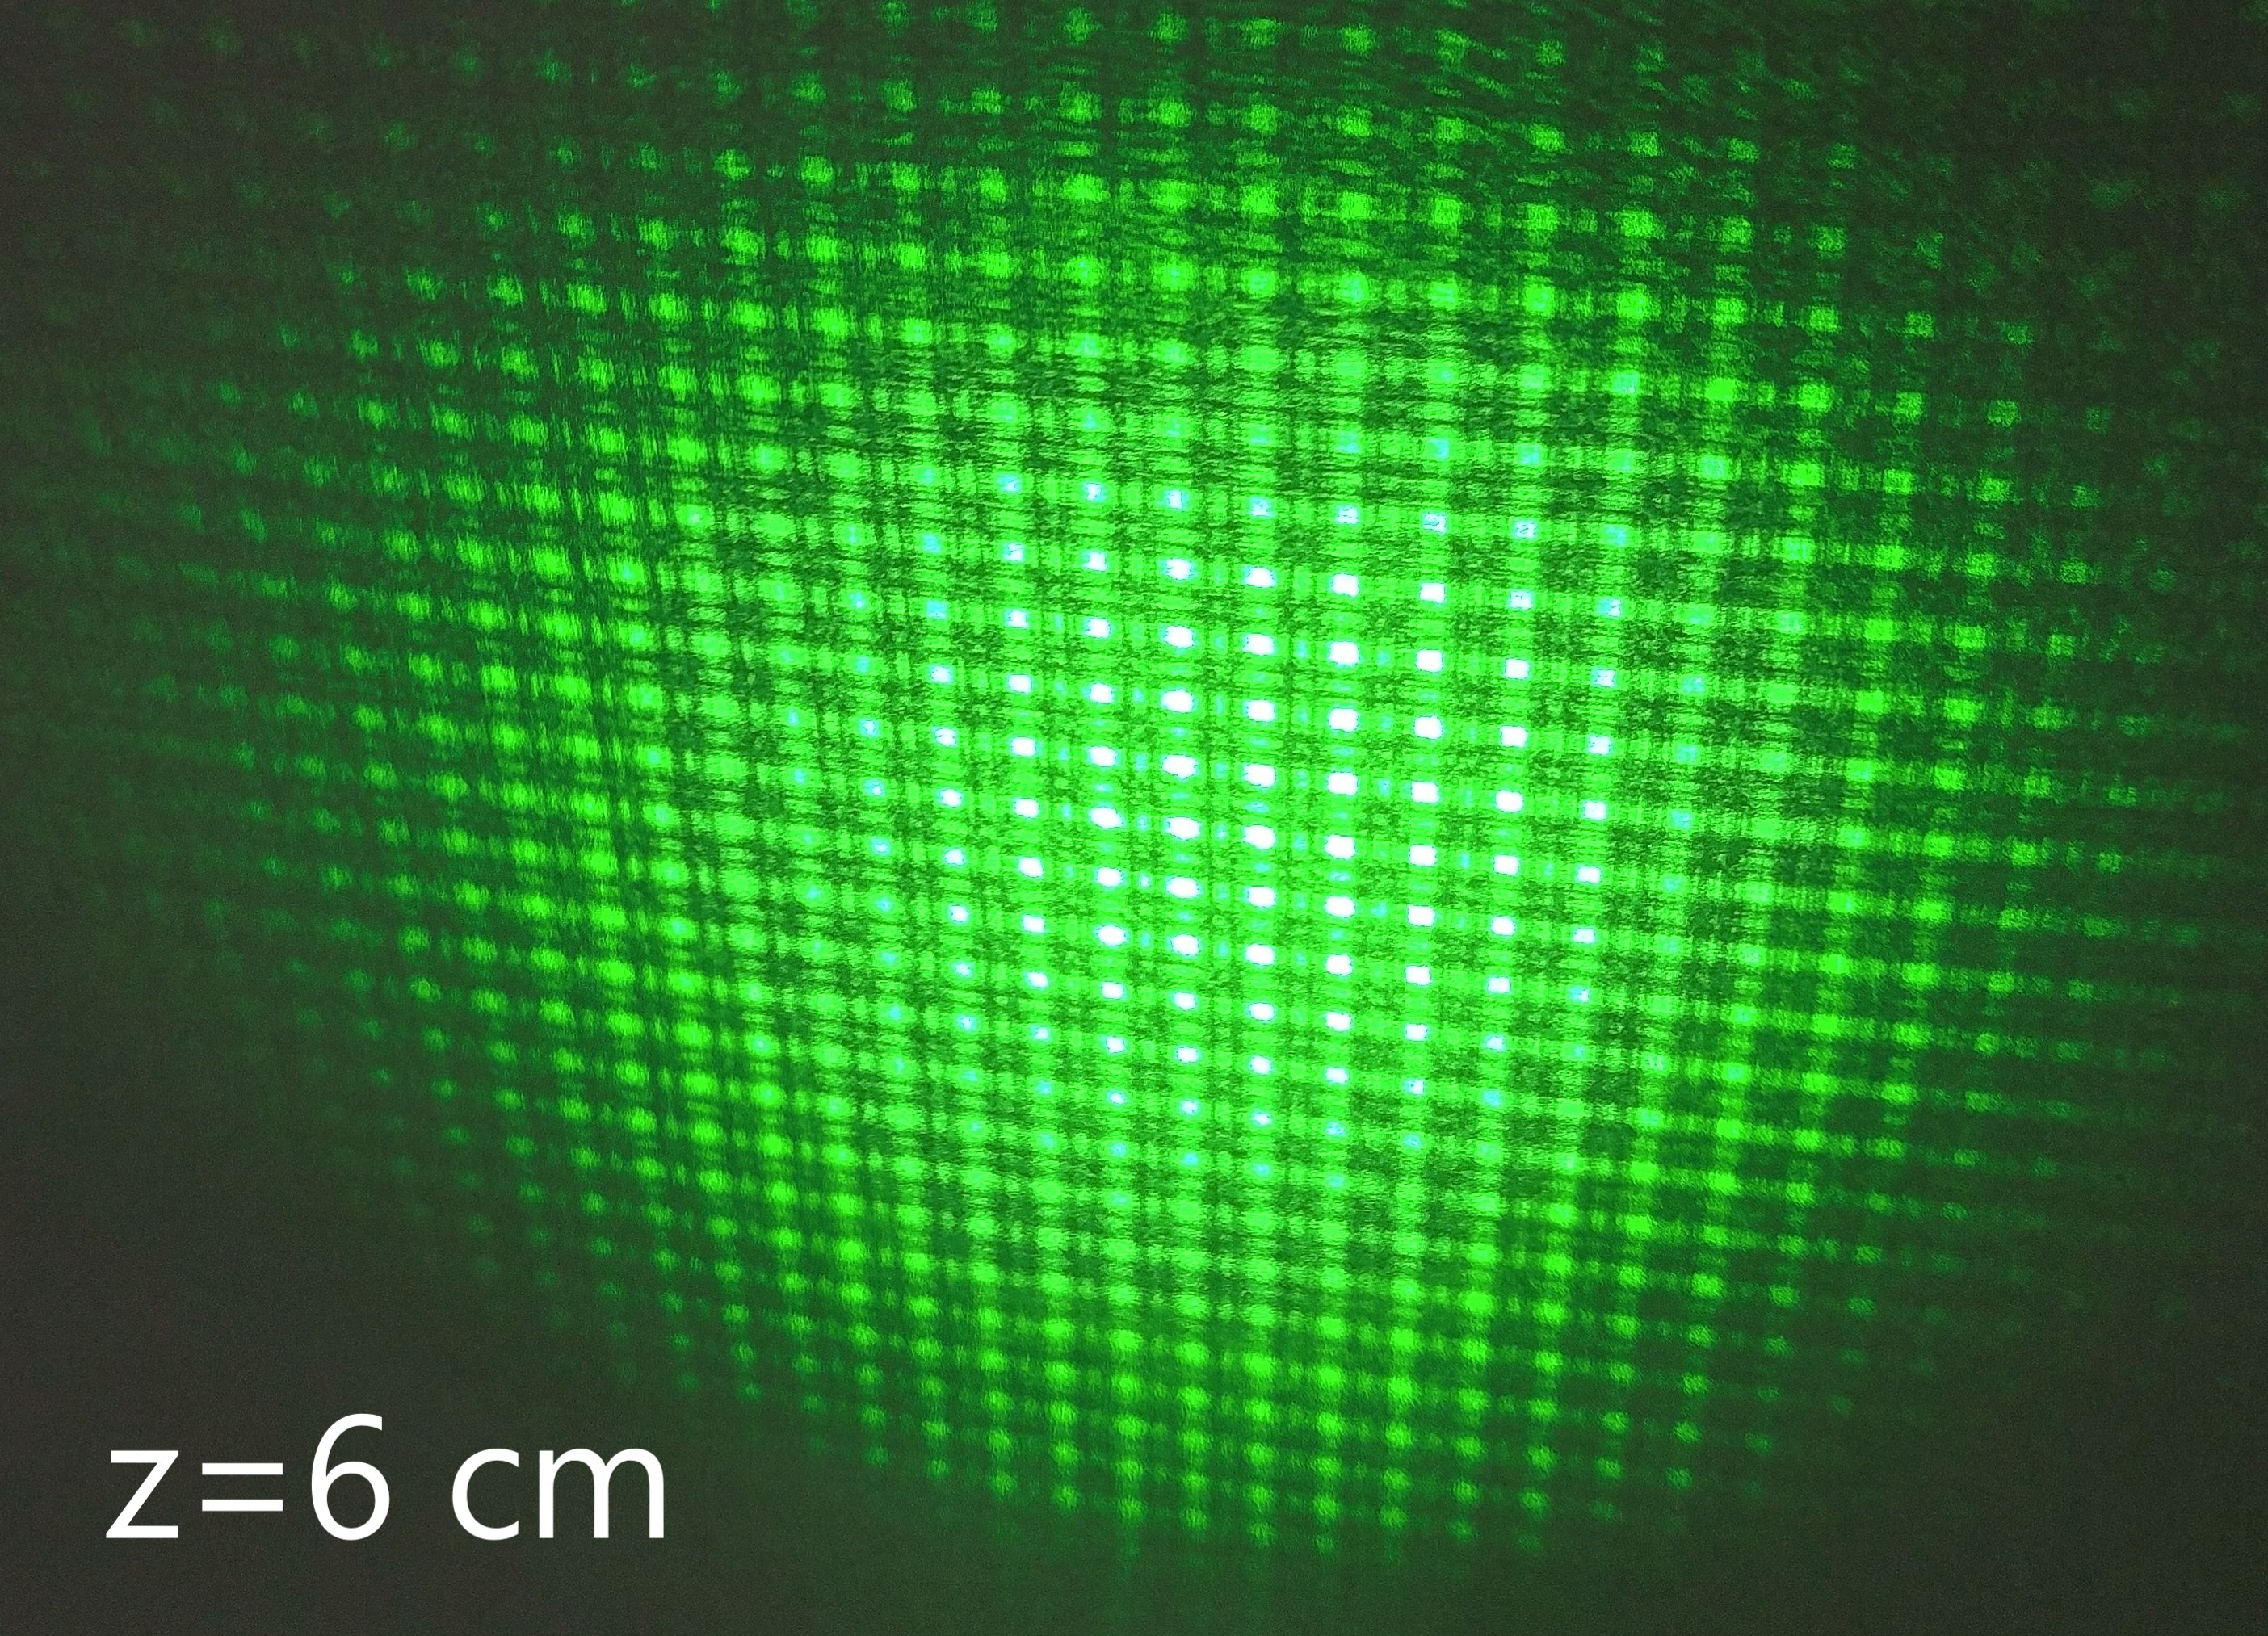
\includegraphics[width=1\linewidth]{41}
\caption{} %% подпись к рисунку
\label{ris:experimoriginal} %% метка рисунка для ссылки на него
\end{minipage}
\hfill 
\begin{minipage}[h]{0.4\linewidth}
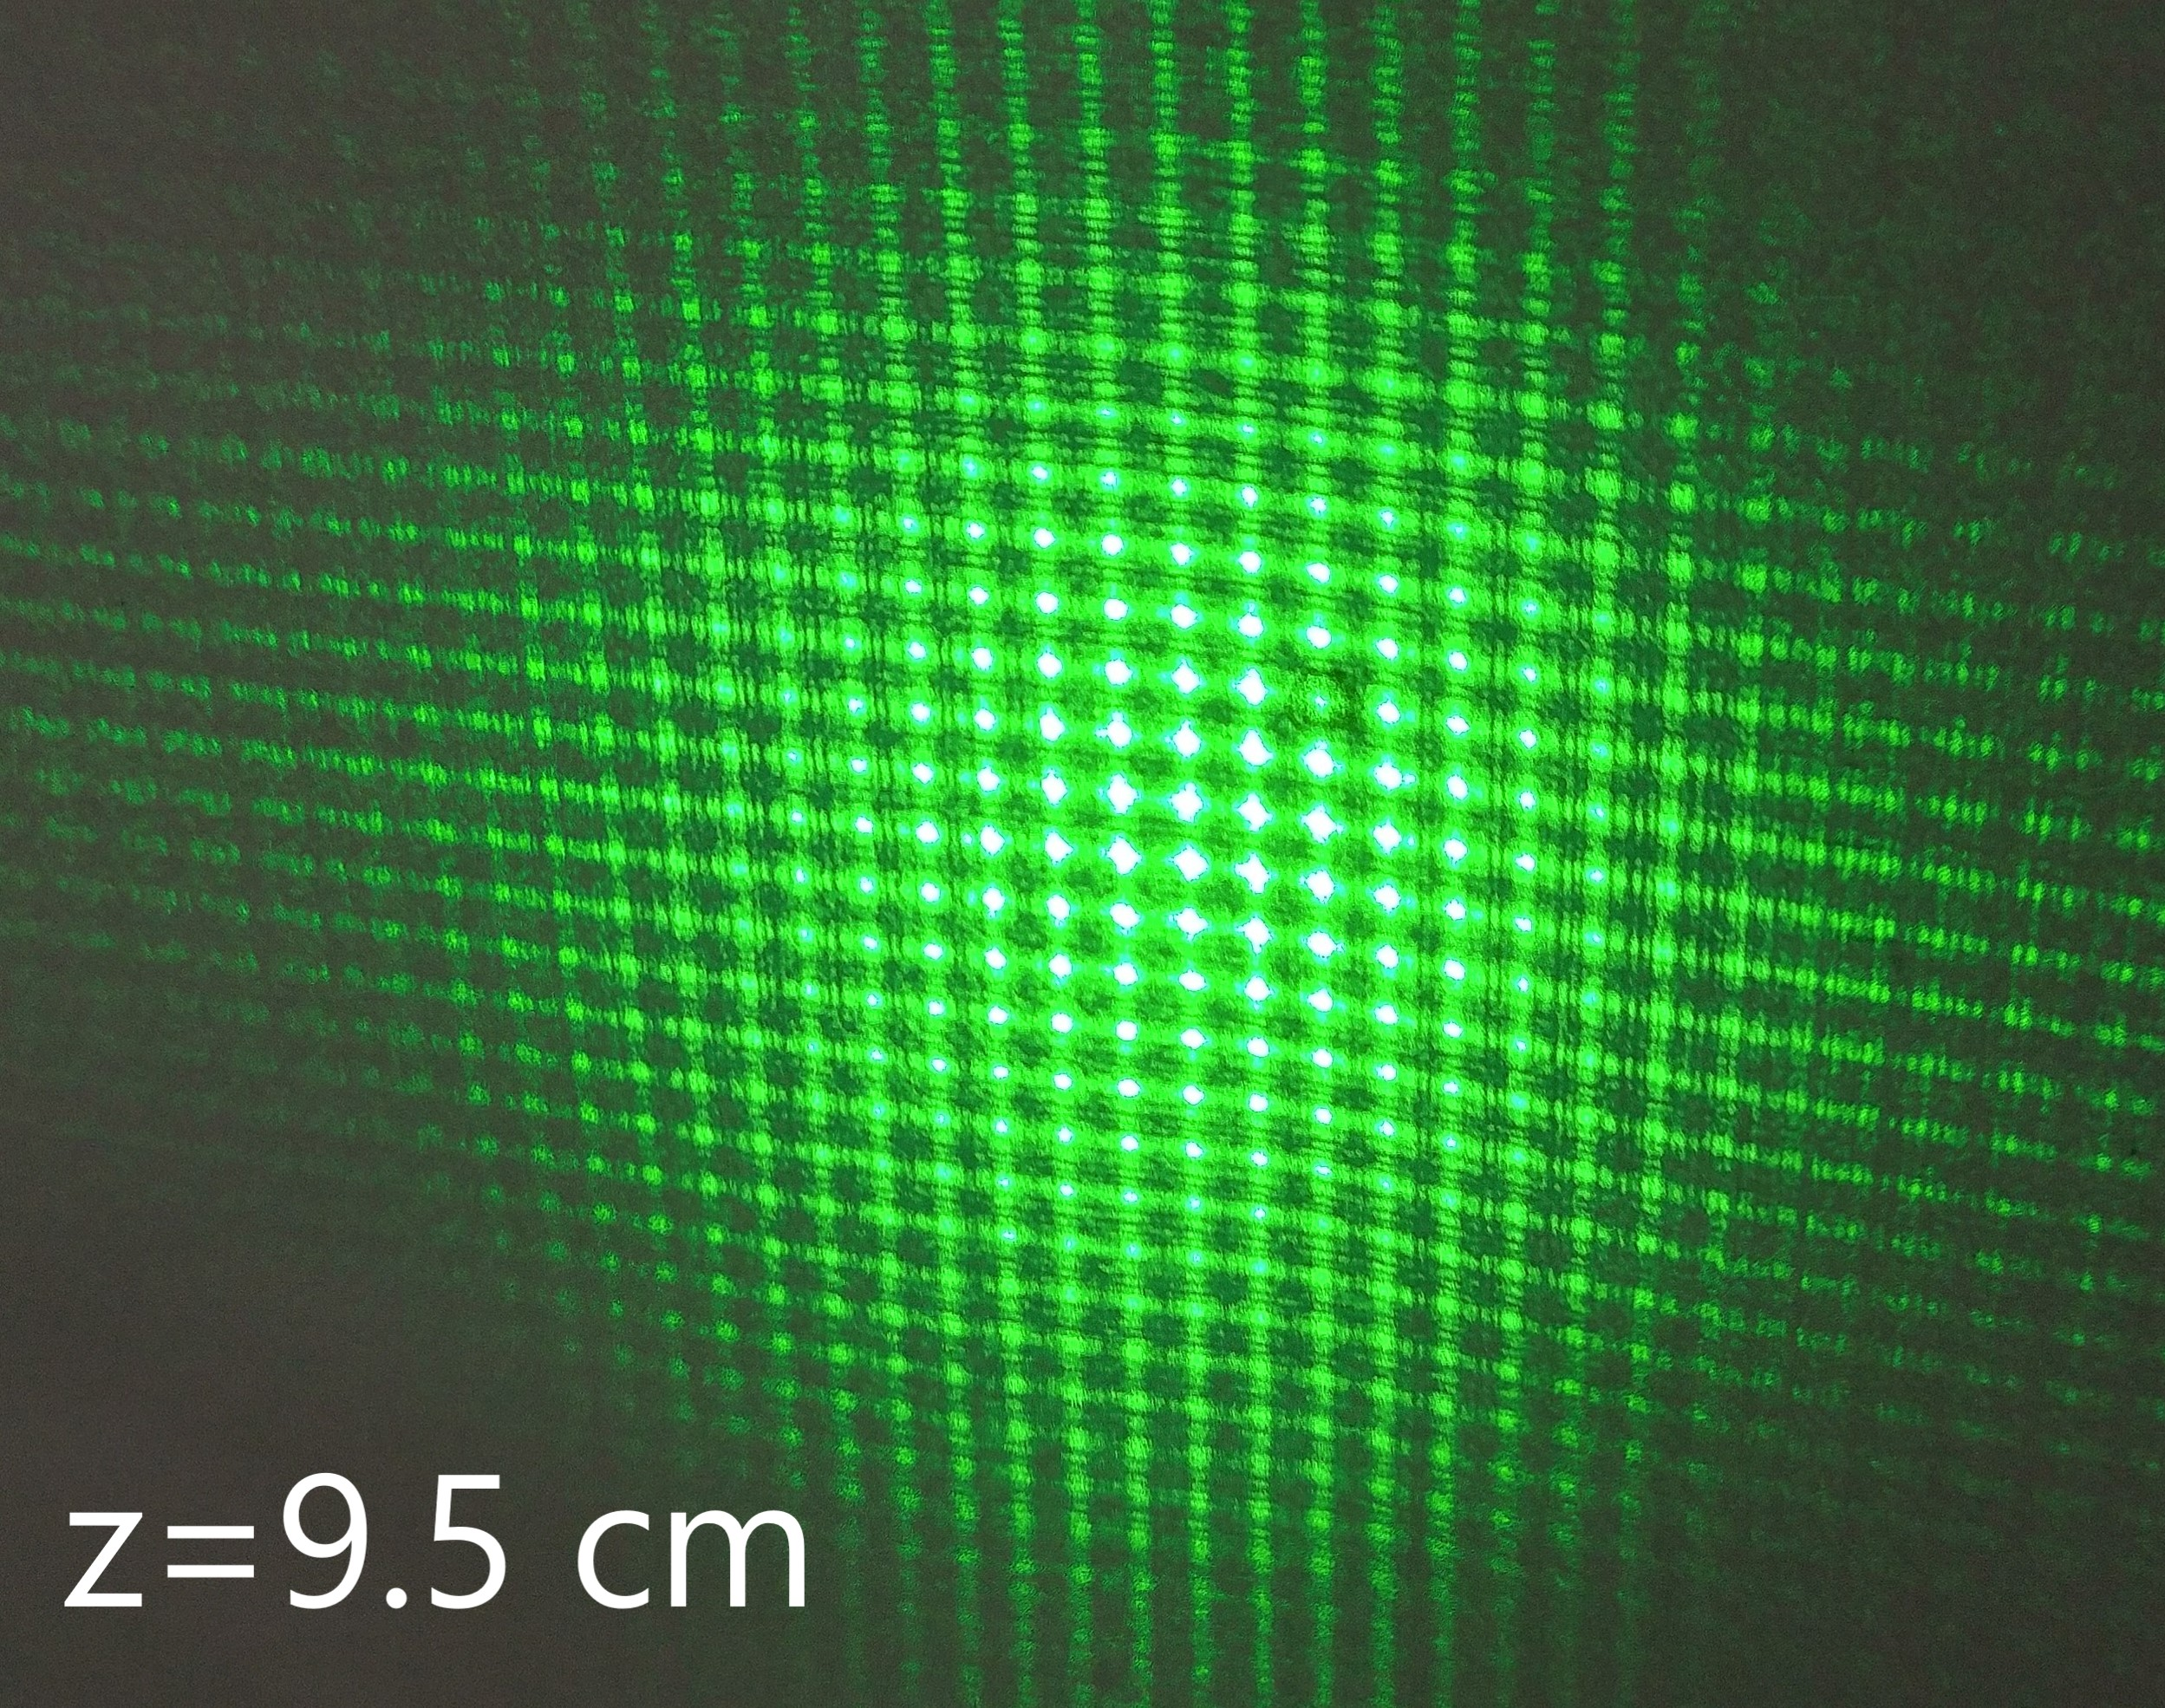
\includegraphics[width=1\linewidth]{42}
\caption{}
\label{ris:experimcoded}
\end{minipage}
\end{center}
\end{figure}
\begin{figure}[h]
\begin{center}
\begin{minipage}[h]{0.4\linewidth}
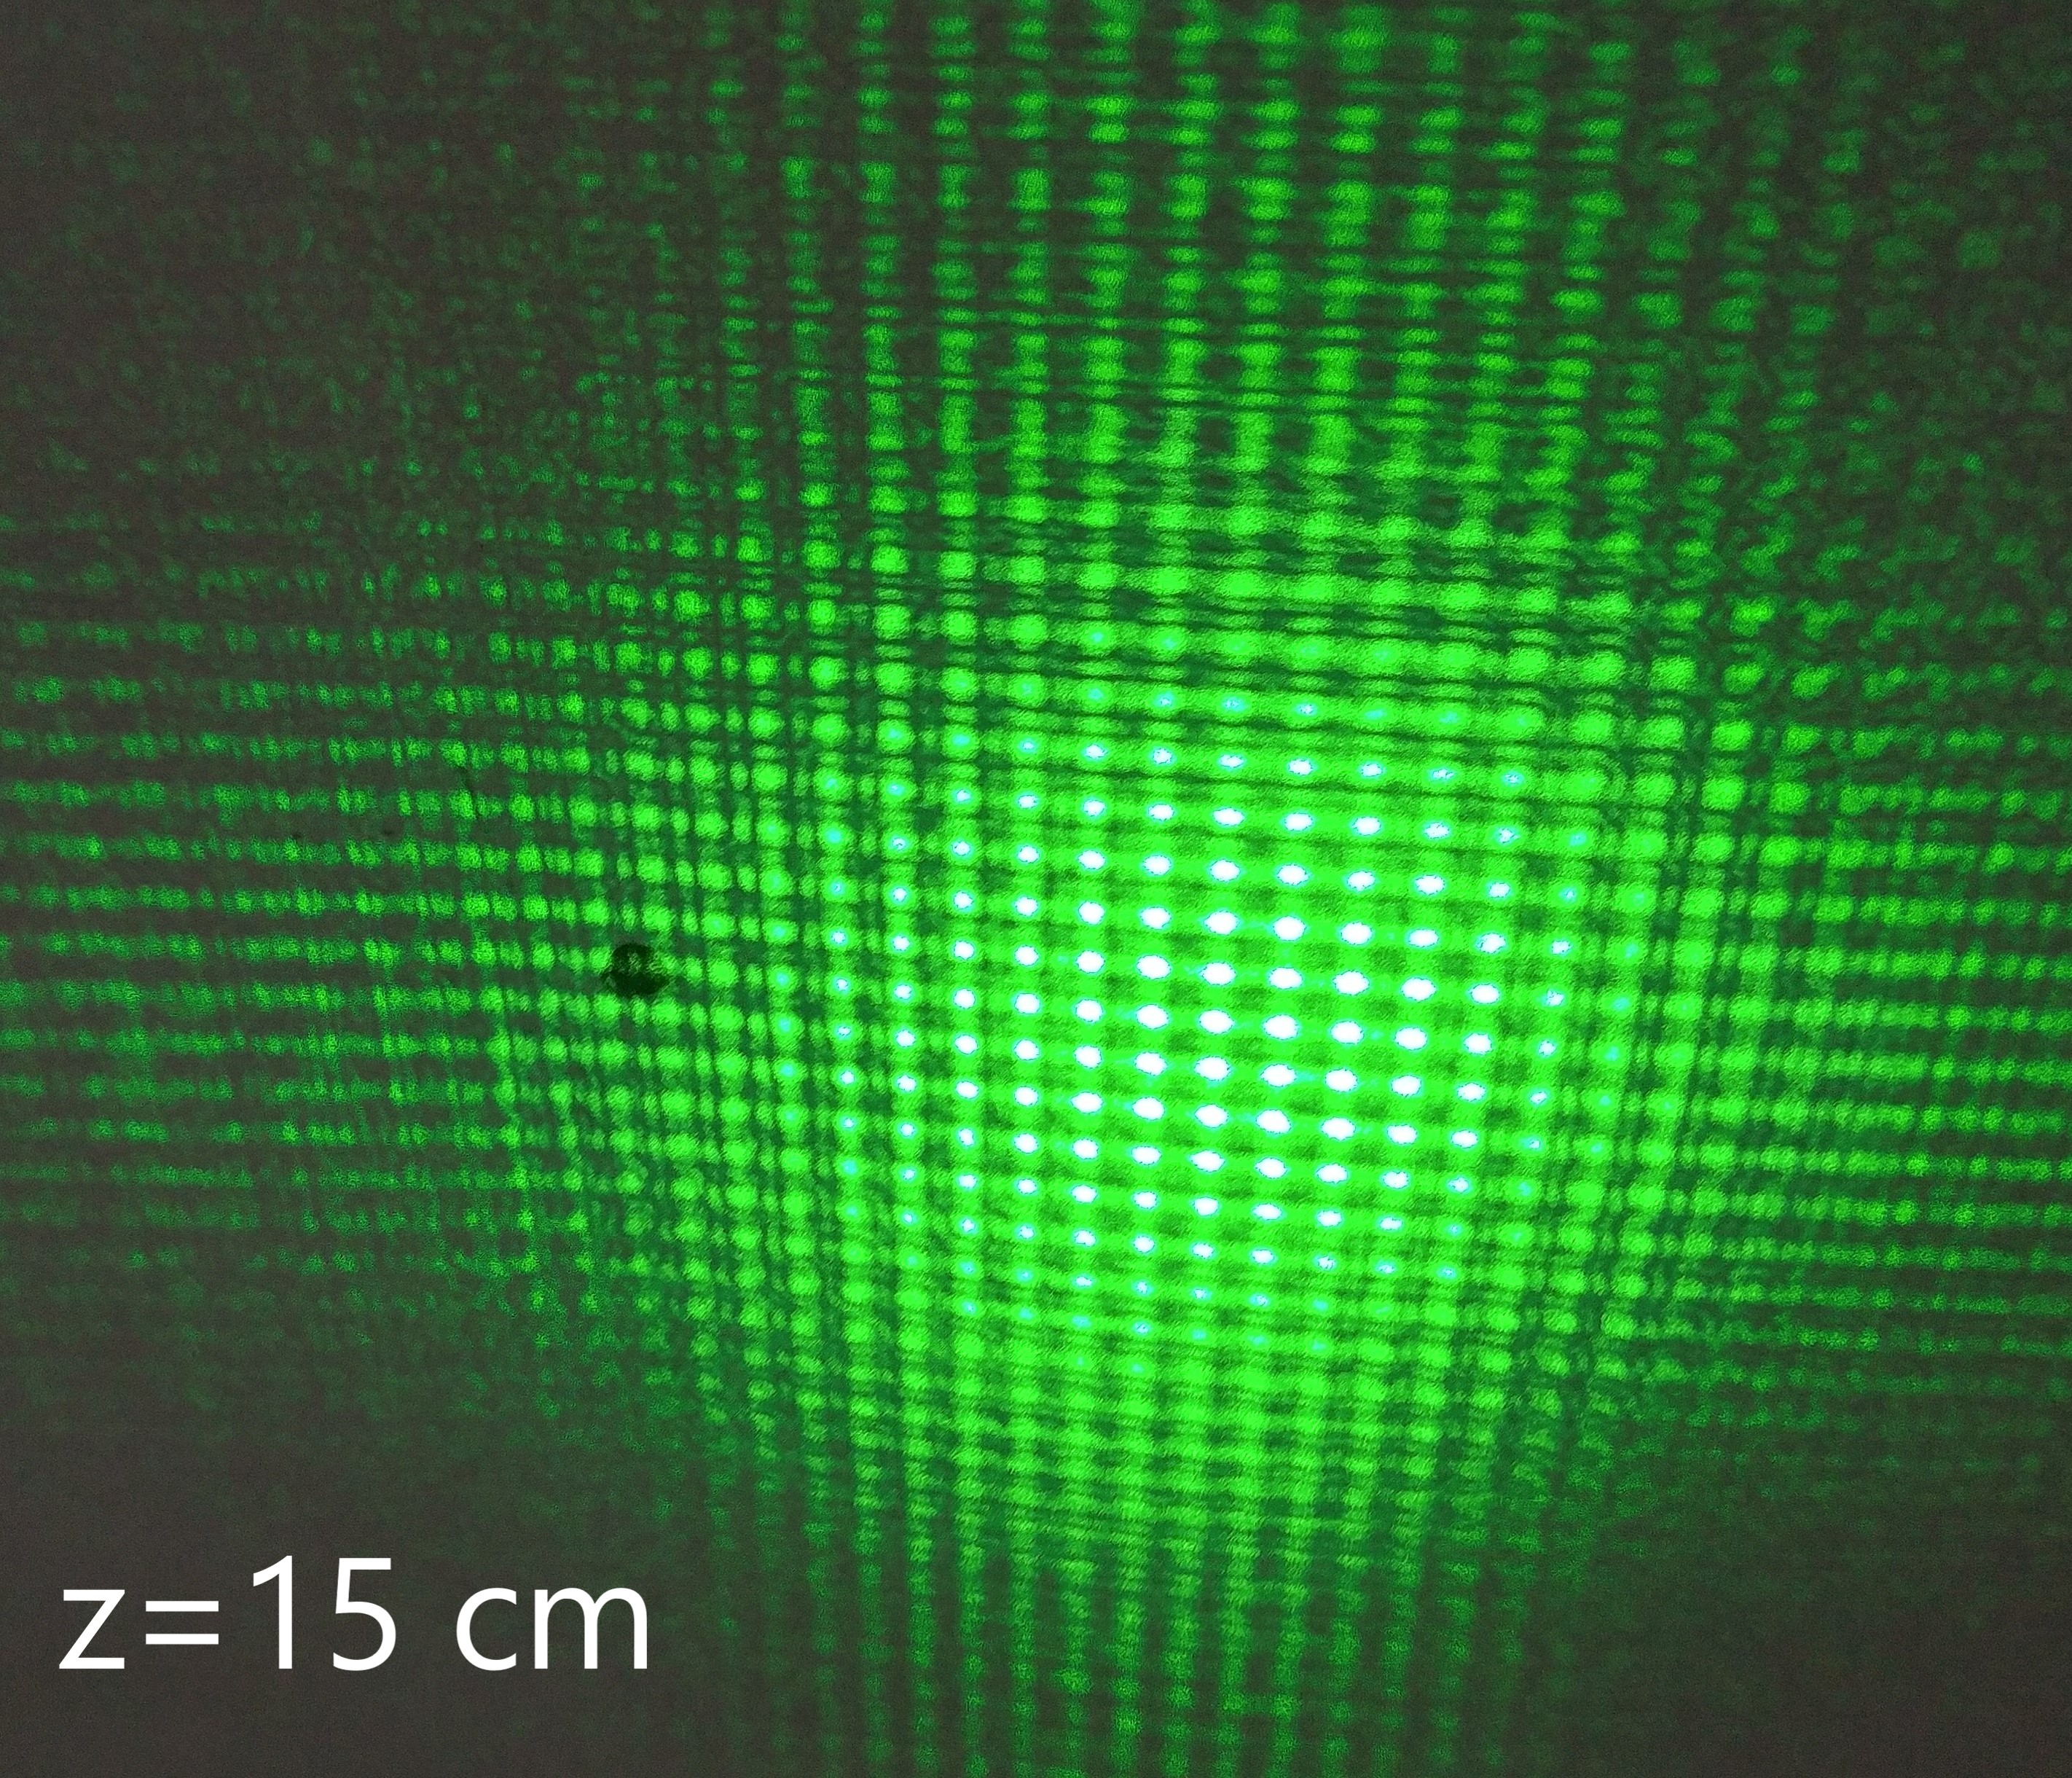
\includegraphics[width=1\linewidth]{43}
\caption{} %% подпись к рисунку
\label{ris:experimoriginal} %% метка рисунка для ссылки на него
\end{minipage}
\hfill 
\begin{minipage}[h]{0.4\linewidth}
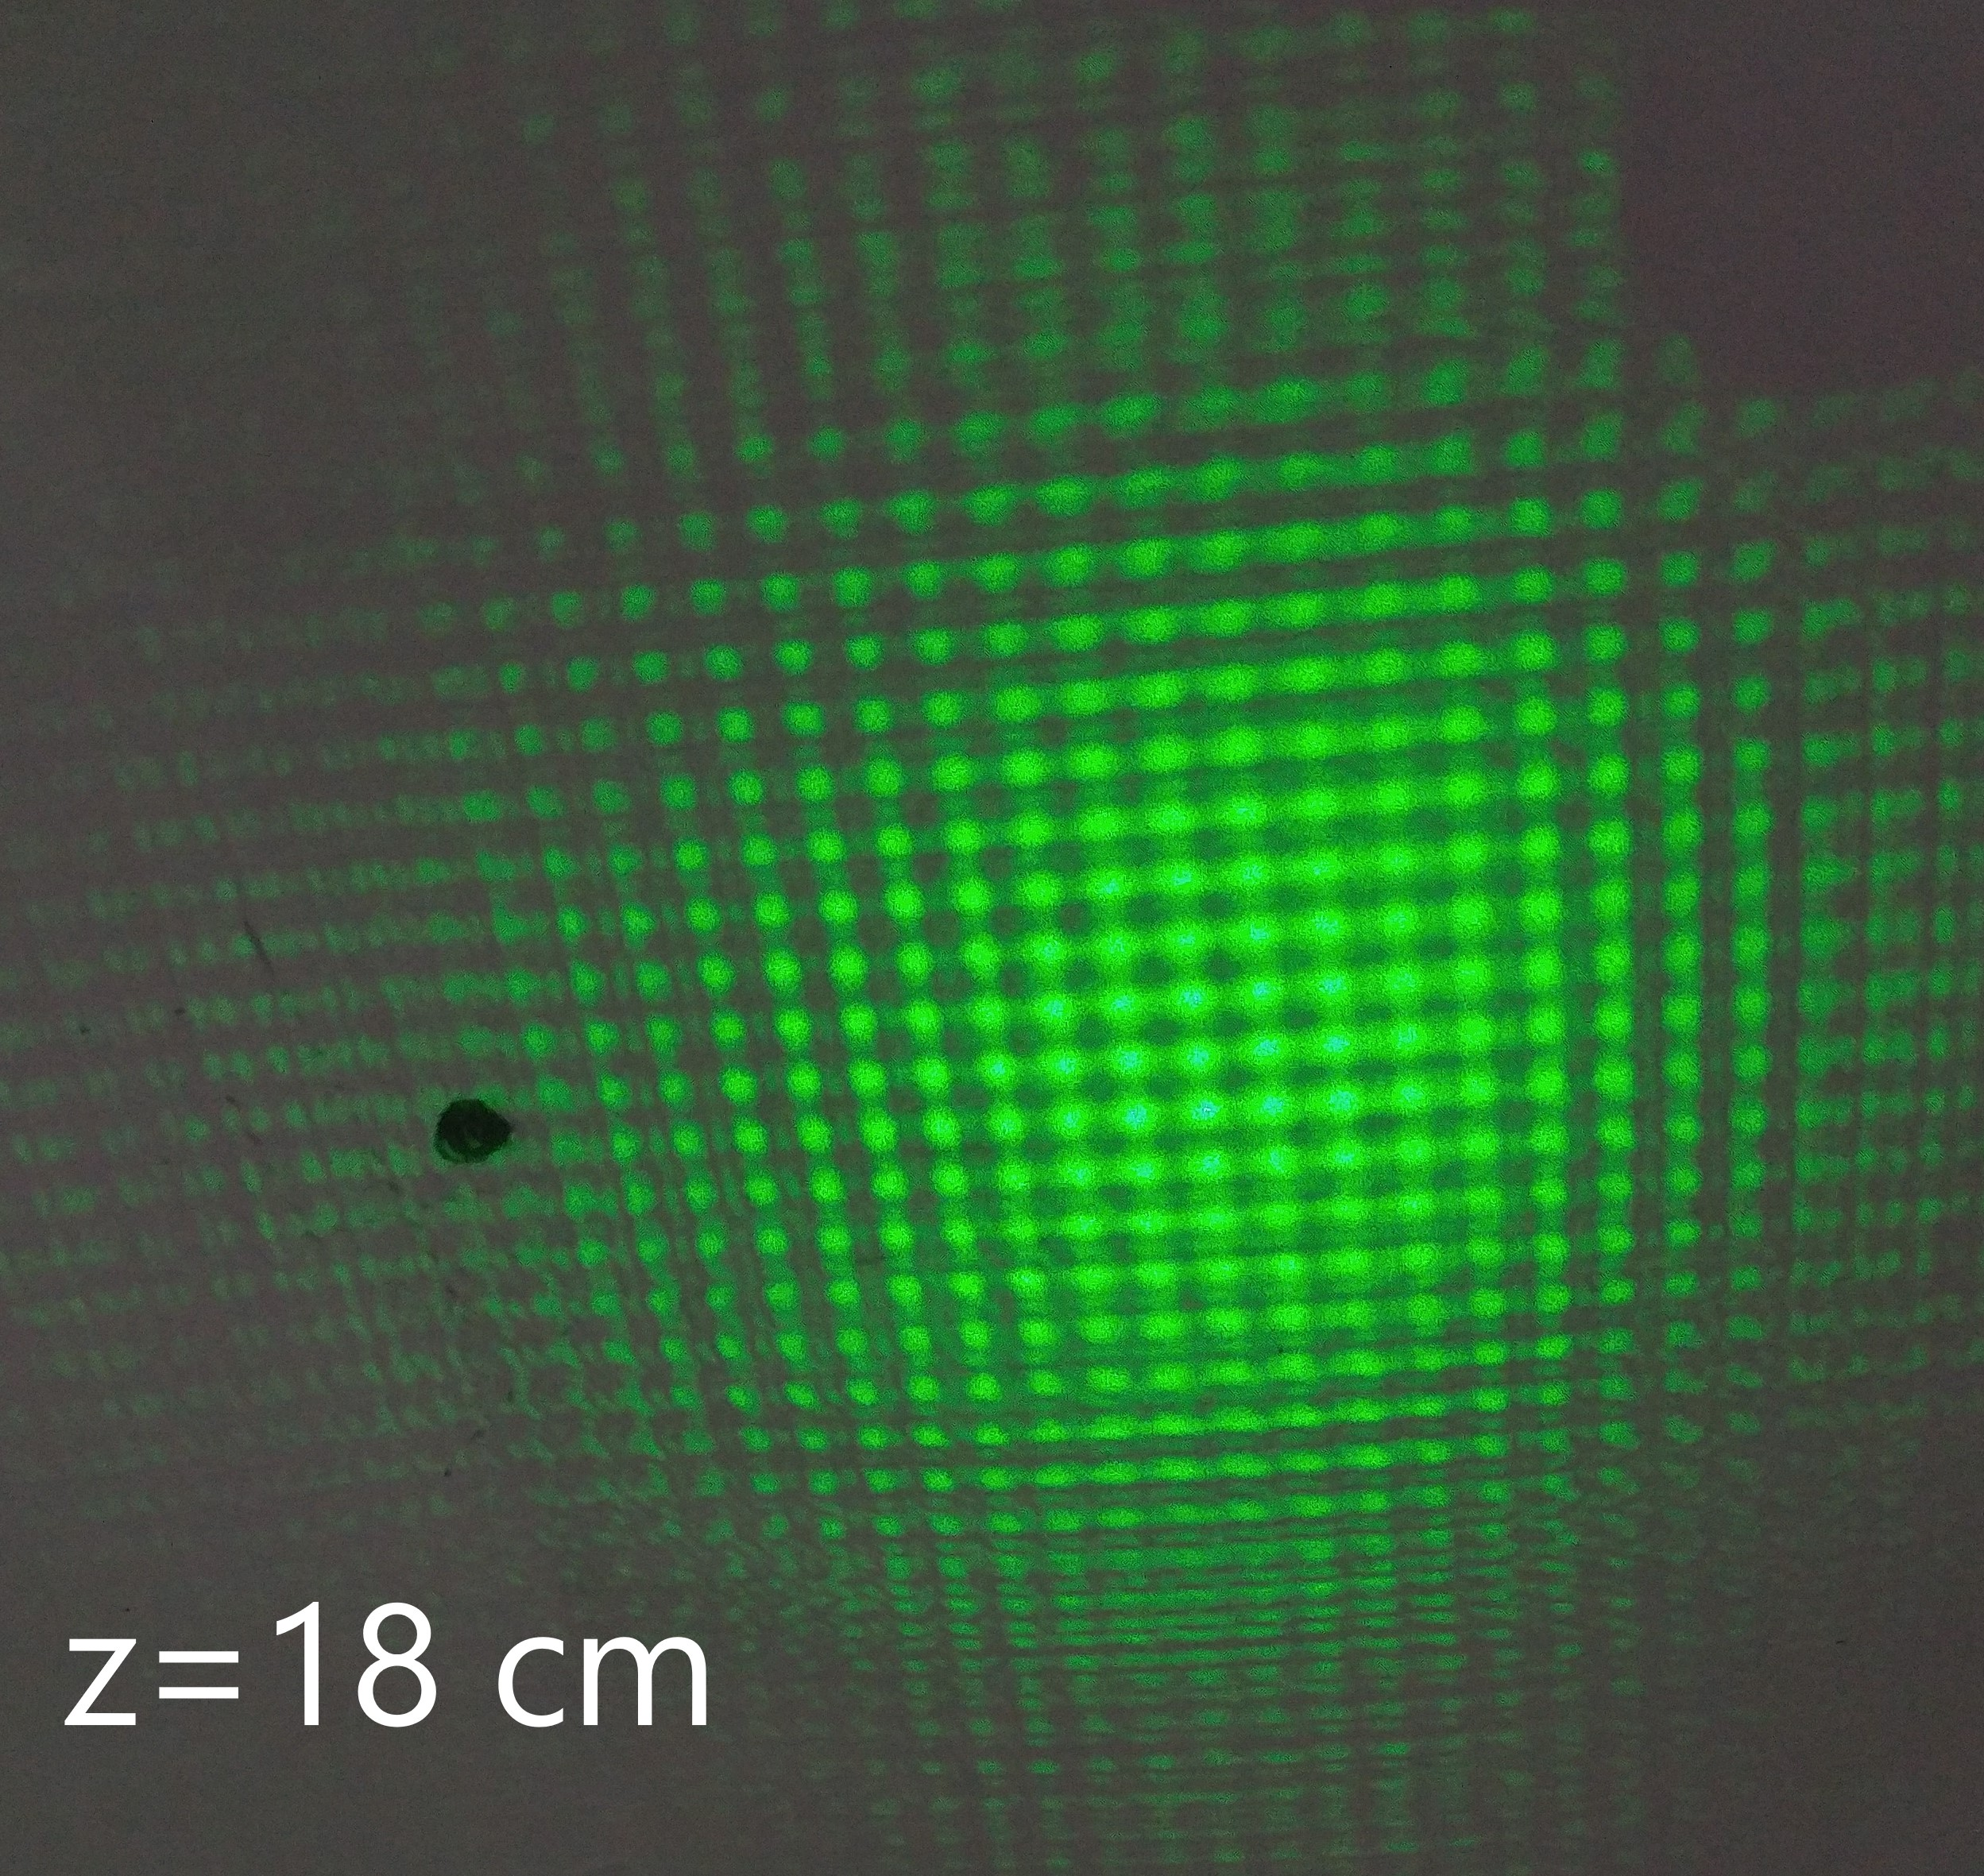
\includegraphics[width=1\linewidth]{44}
\caption{}
\label{ris:experimcoded}
\end{minipage}
\end{center}
\end{figure}
\begin{figure}[h]
\begin{center}
\begin{minipage}[h]{0.4\linewidth}
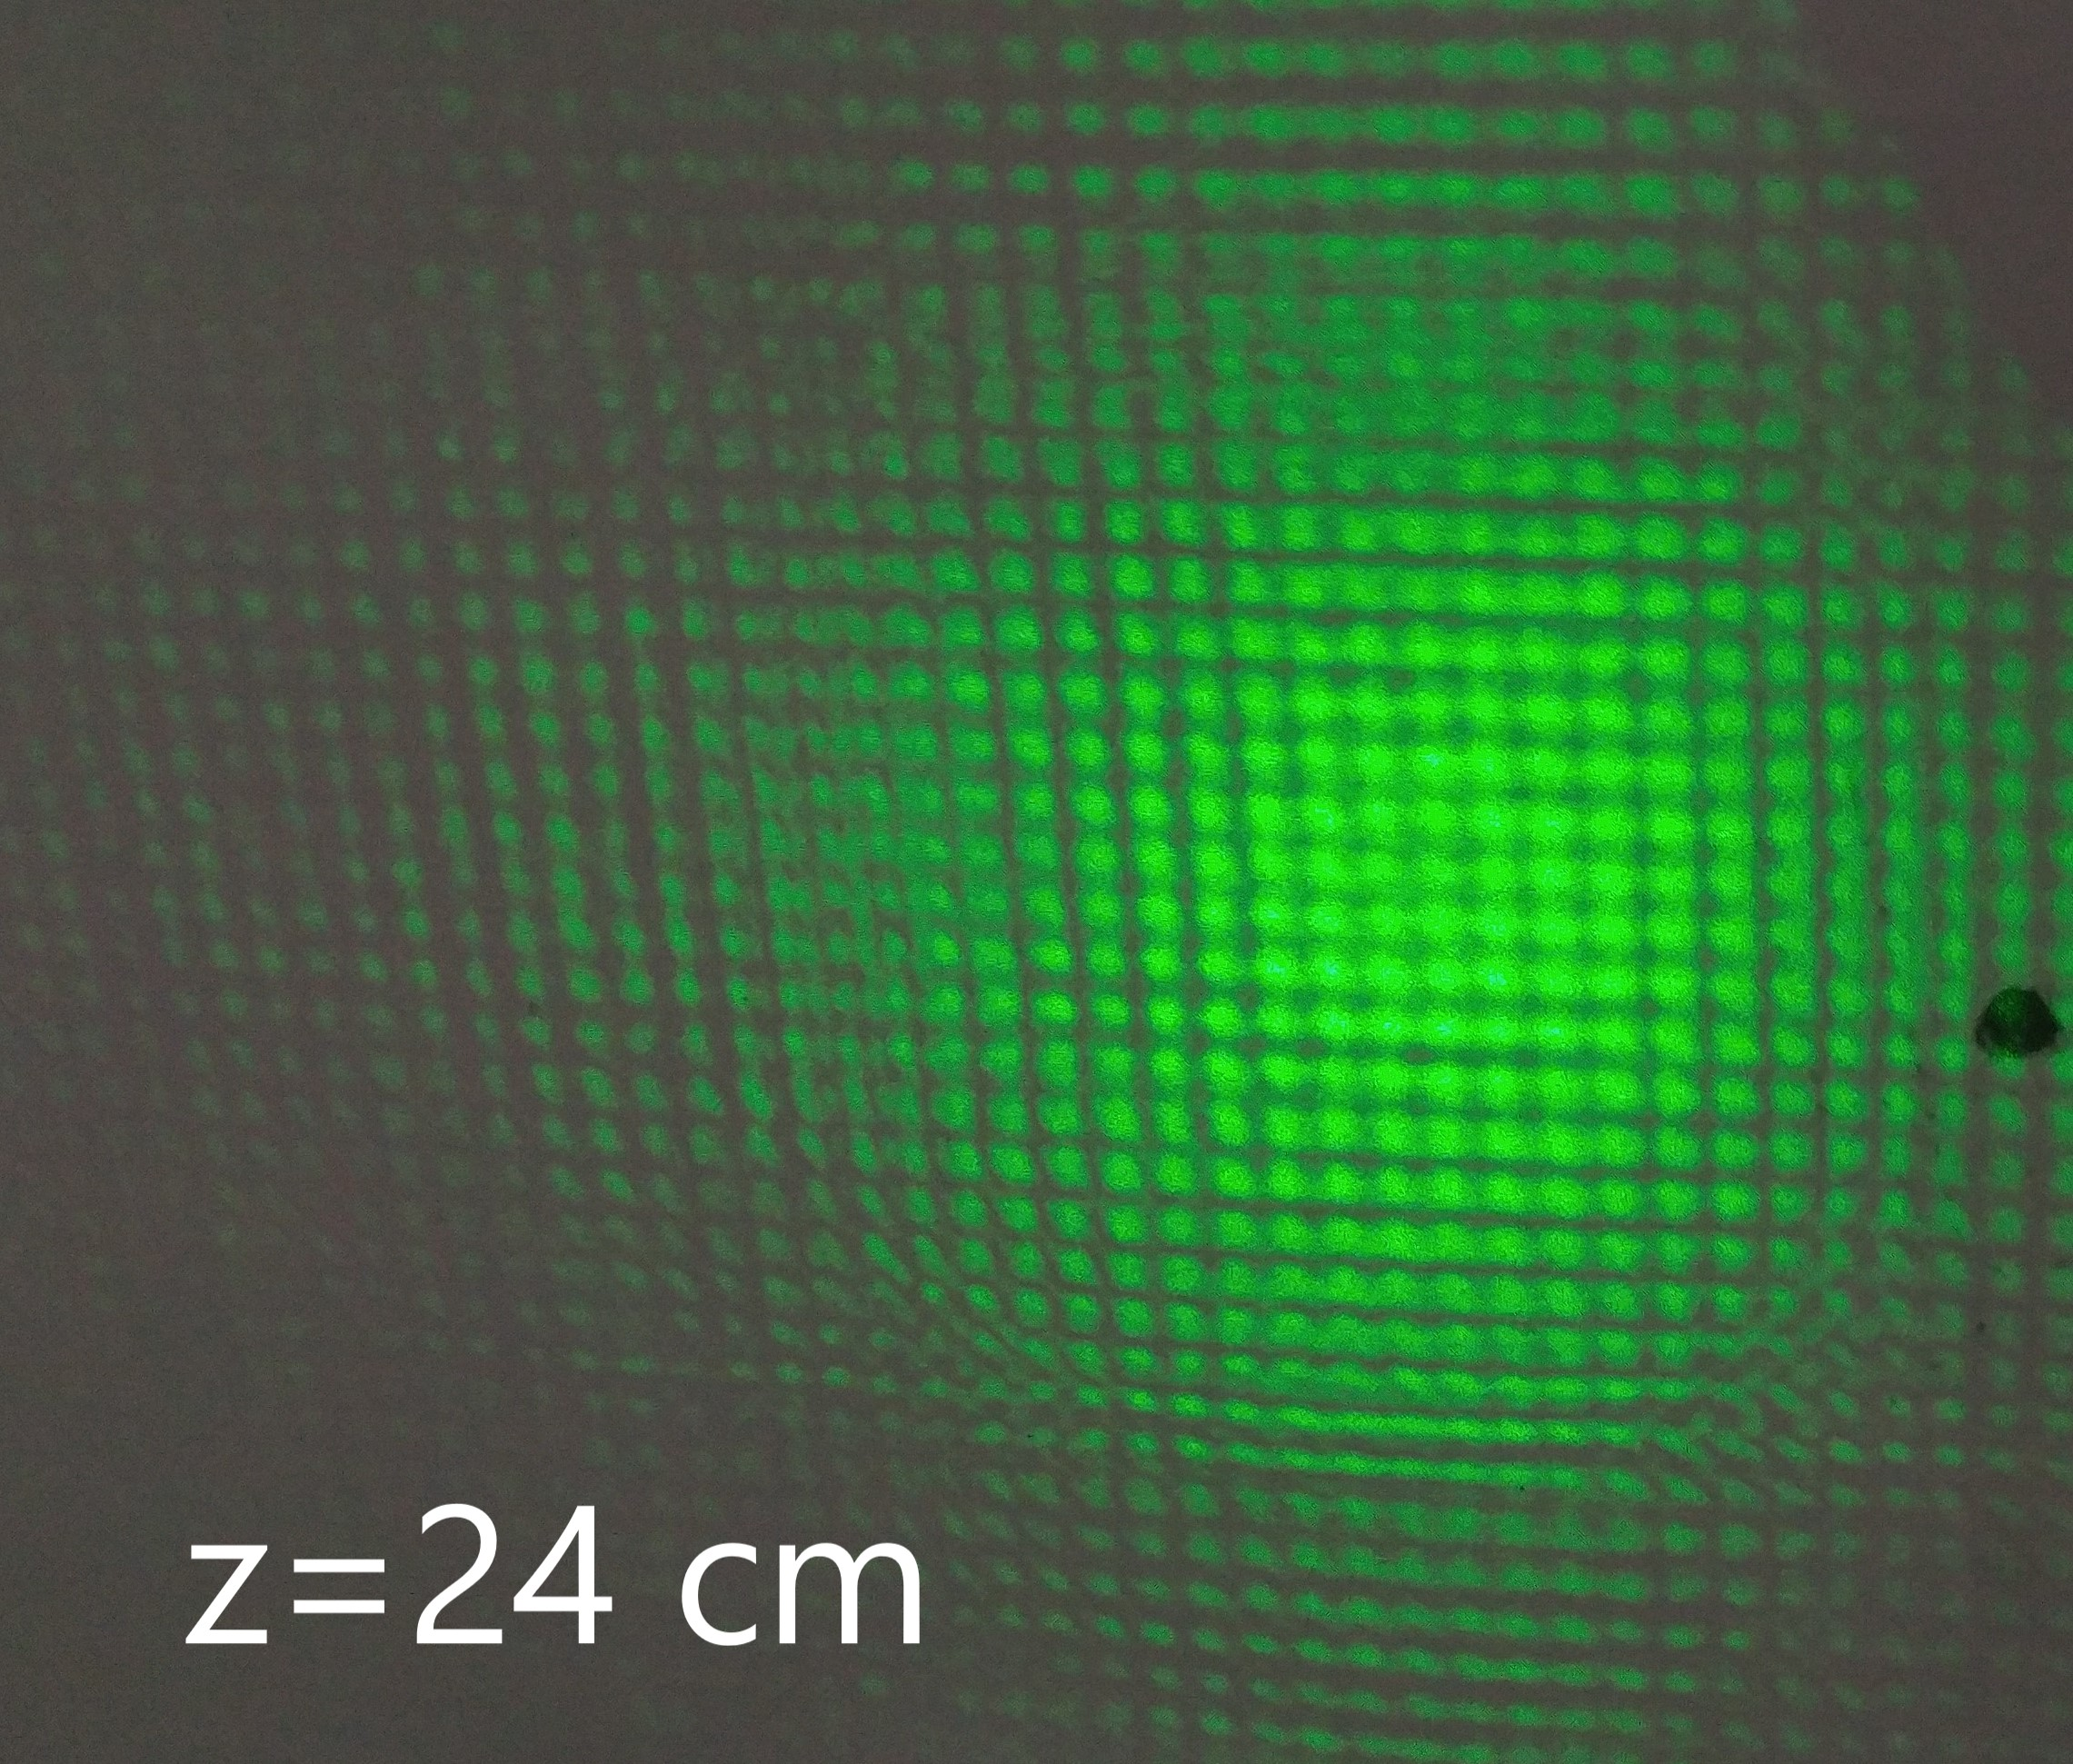
\includegraphics[width=1\linewidth]{45}
\caption{} %% подпись к рисунку
\label{ris:experimoriginal} %% метка рисунка для ссылки на него
\end{minipage}
\hfill 
\begin{minipage}[h]{0.4\linewidth}
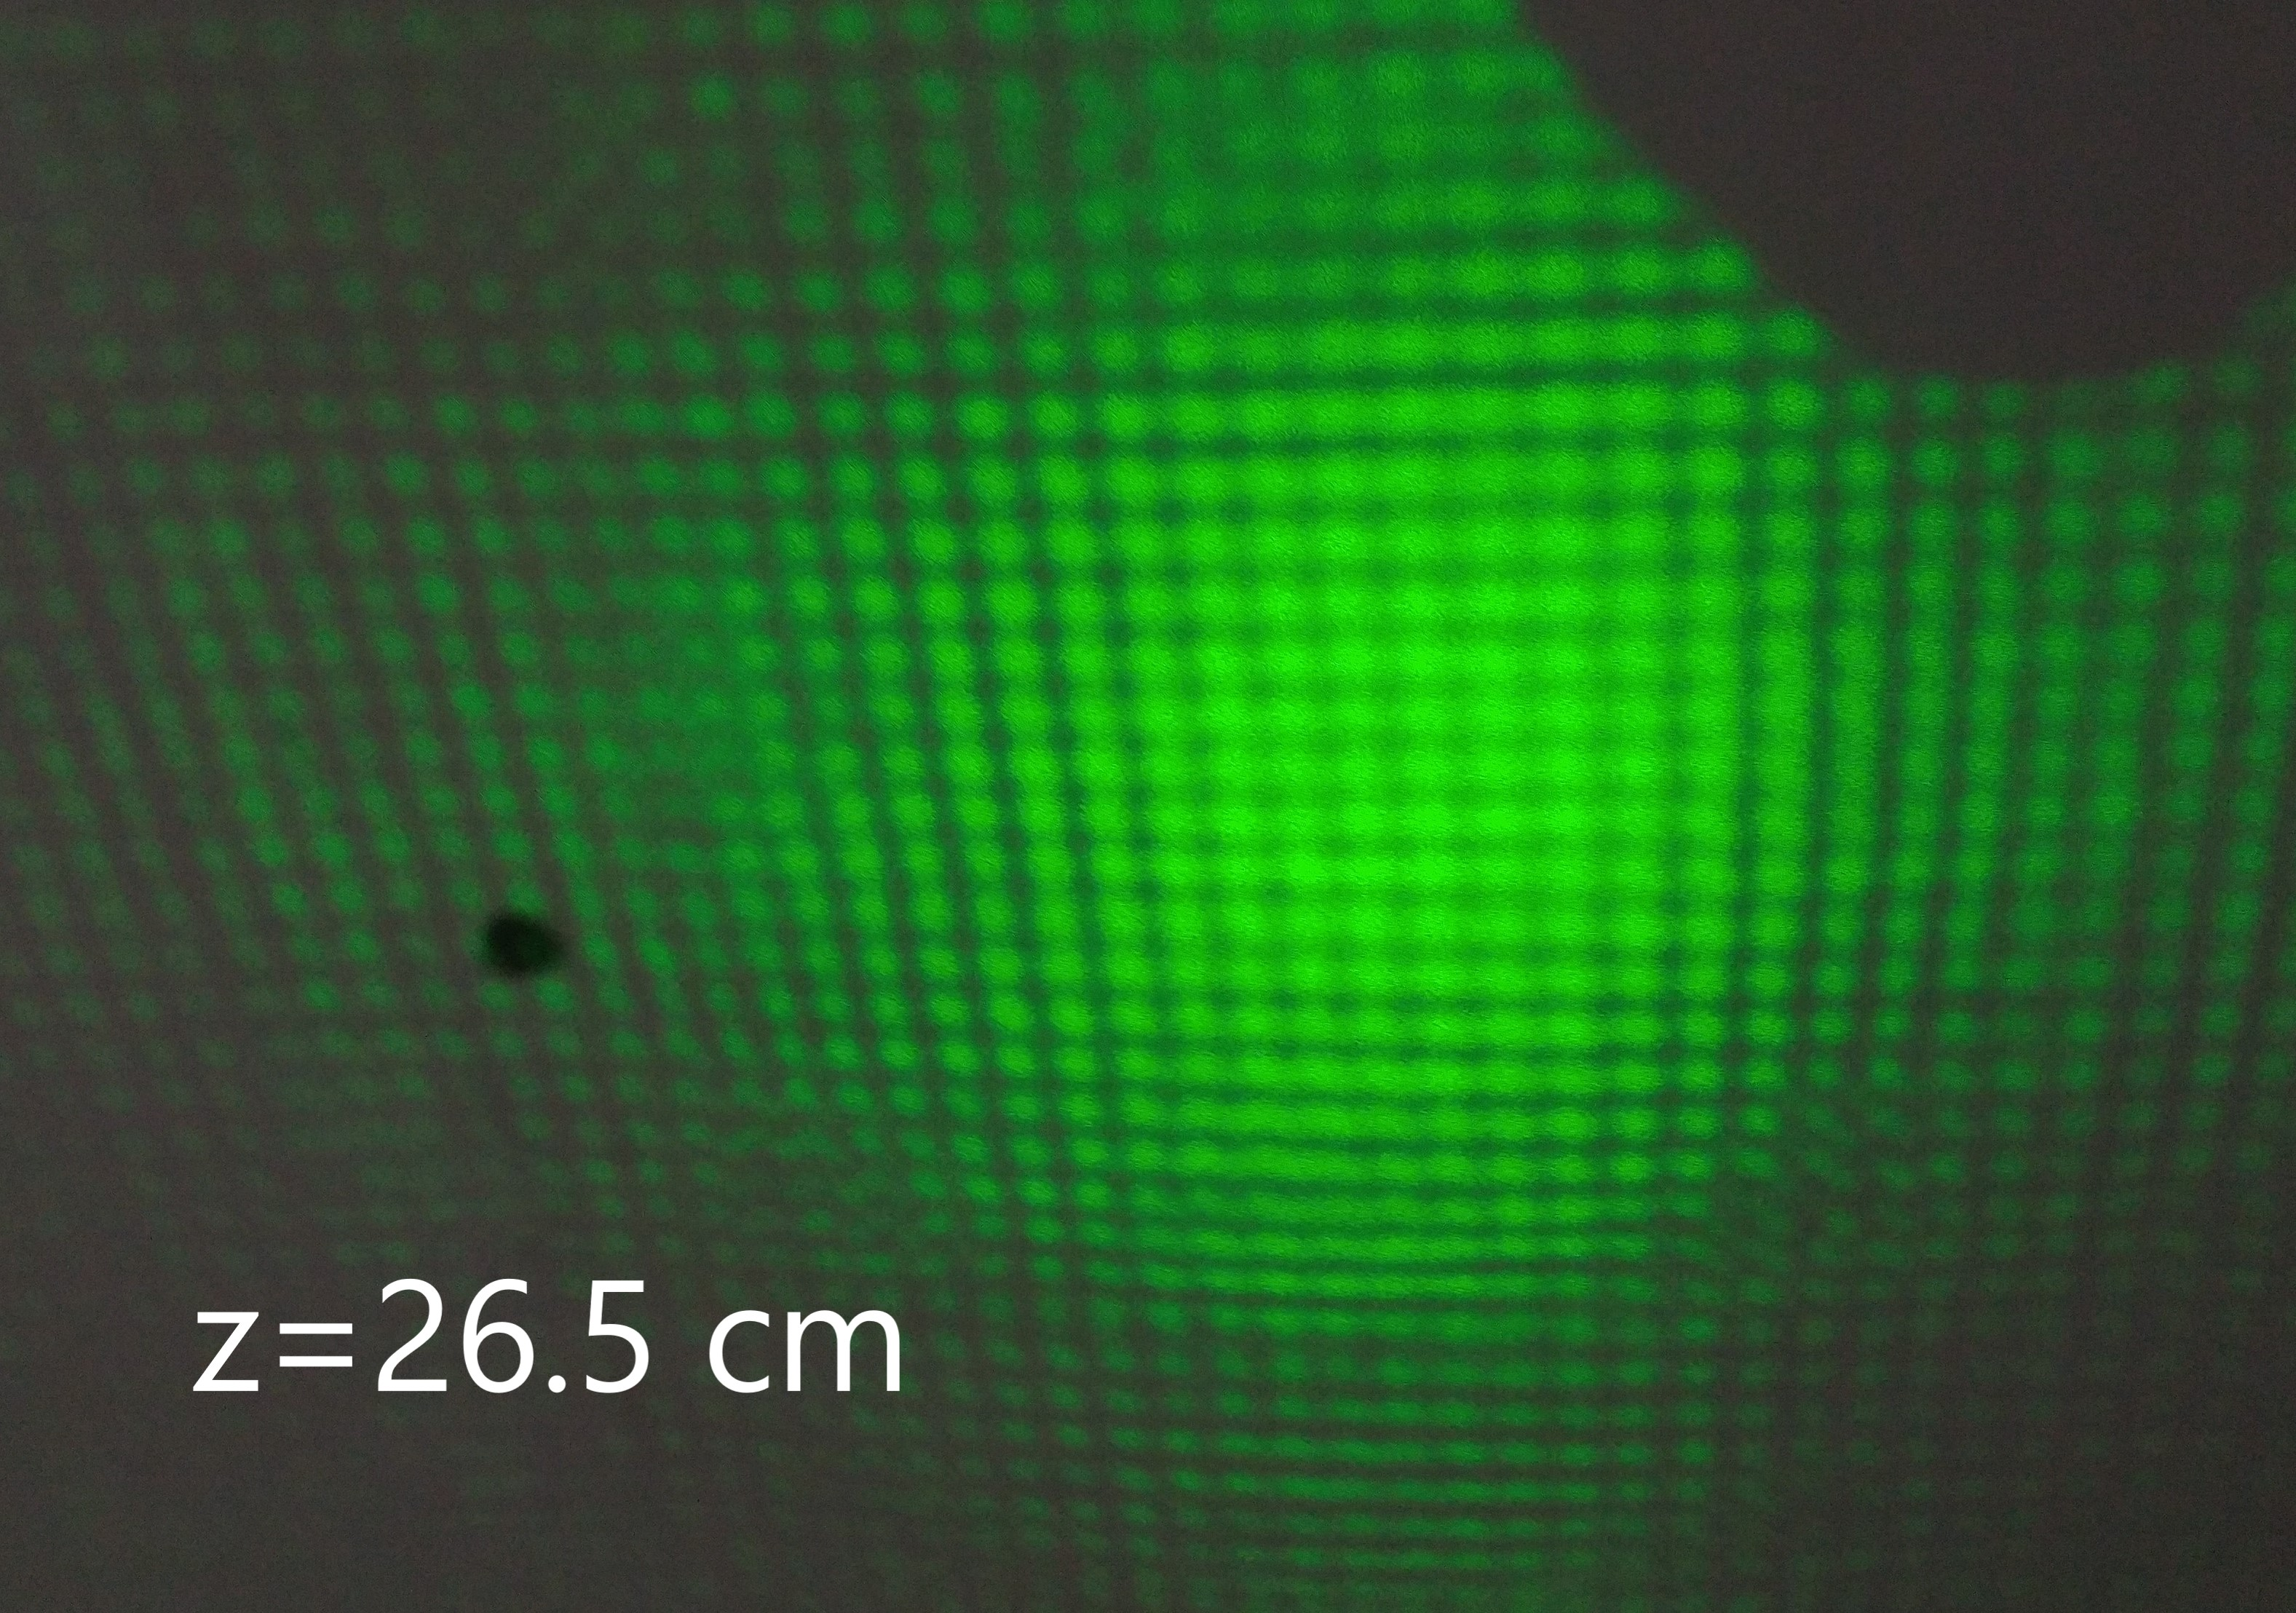
\includegraphics[width=1\linewidth]{46}
\caption{}
\label{ris:experimcoded}
\end{minipage}
\end{center}
\end{figure}
\begin{figure}[h]
\begin{center}
\begin{minipage}[h]{0.4\linewidth}
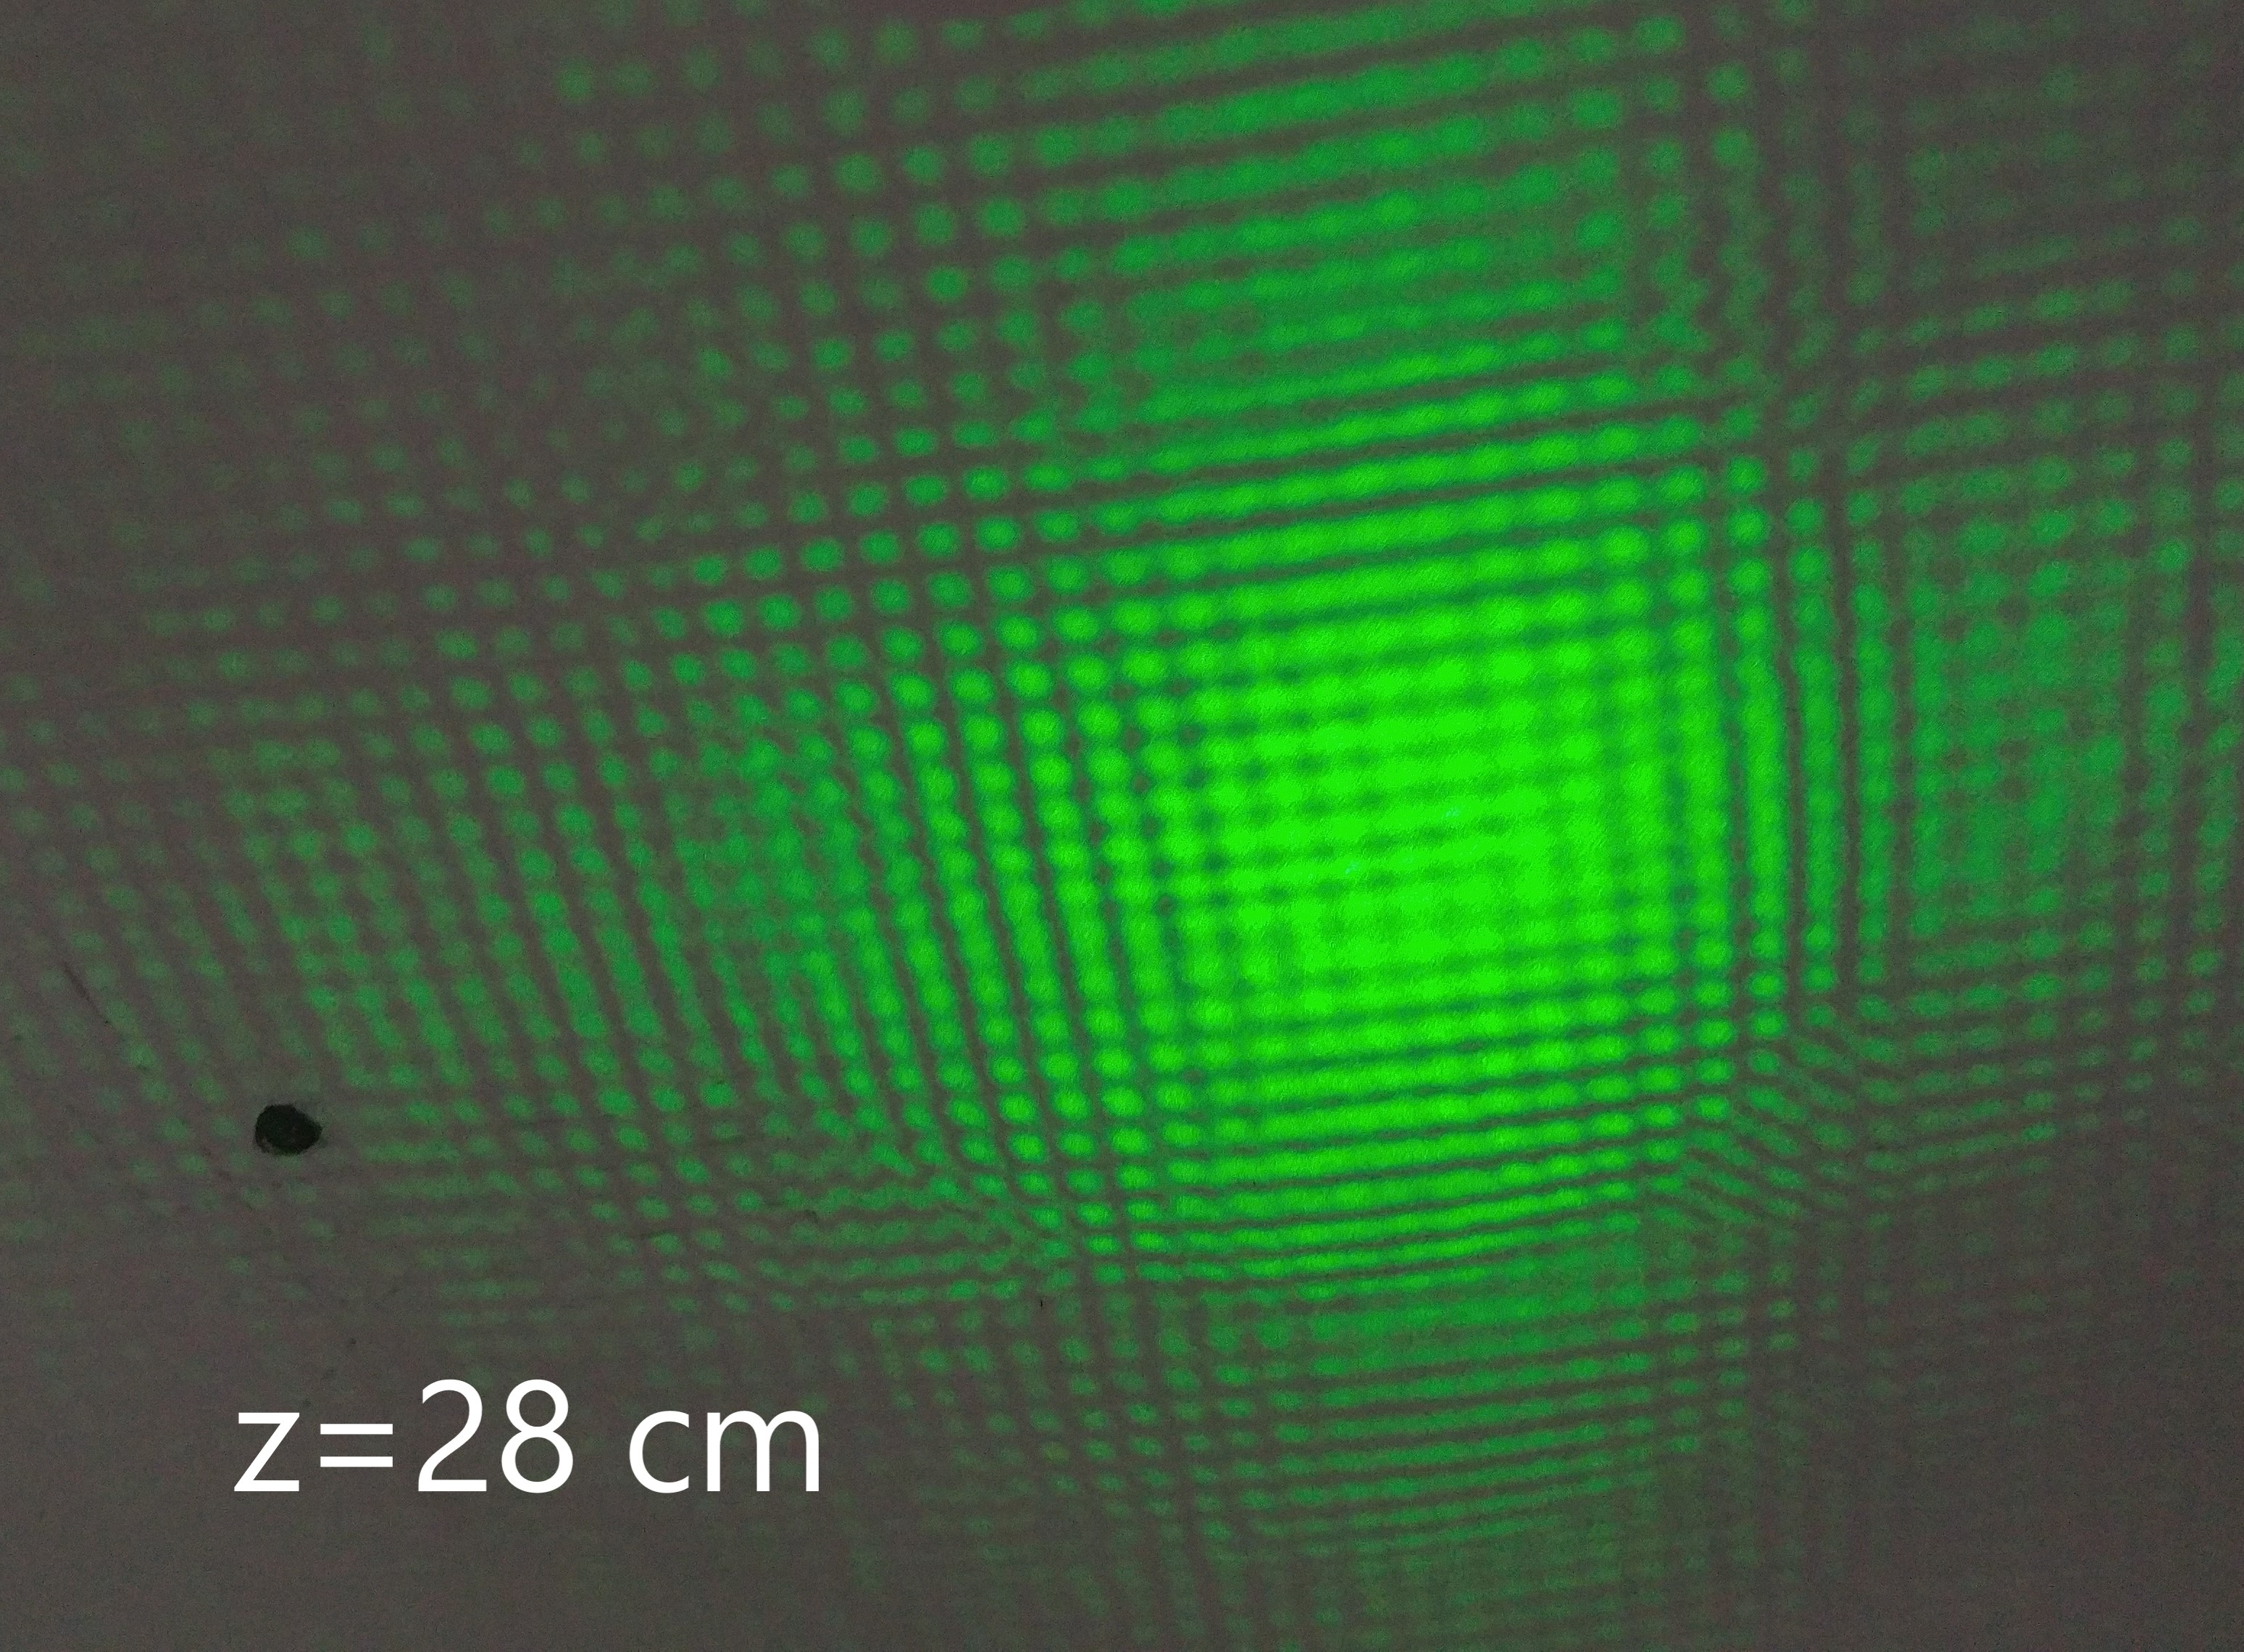
\includegraphics[width=1\linewidth]{47}
\caption{} %% подпись к рисунку
\label{ris:experimoriginal} %% метка рисунка для ссылки на него
\end{minipage}
\hfill 
\begin{minipage}[h]{0.4\linewidth}
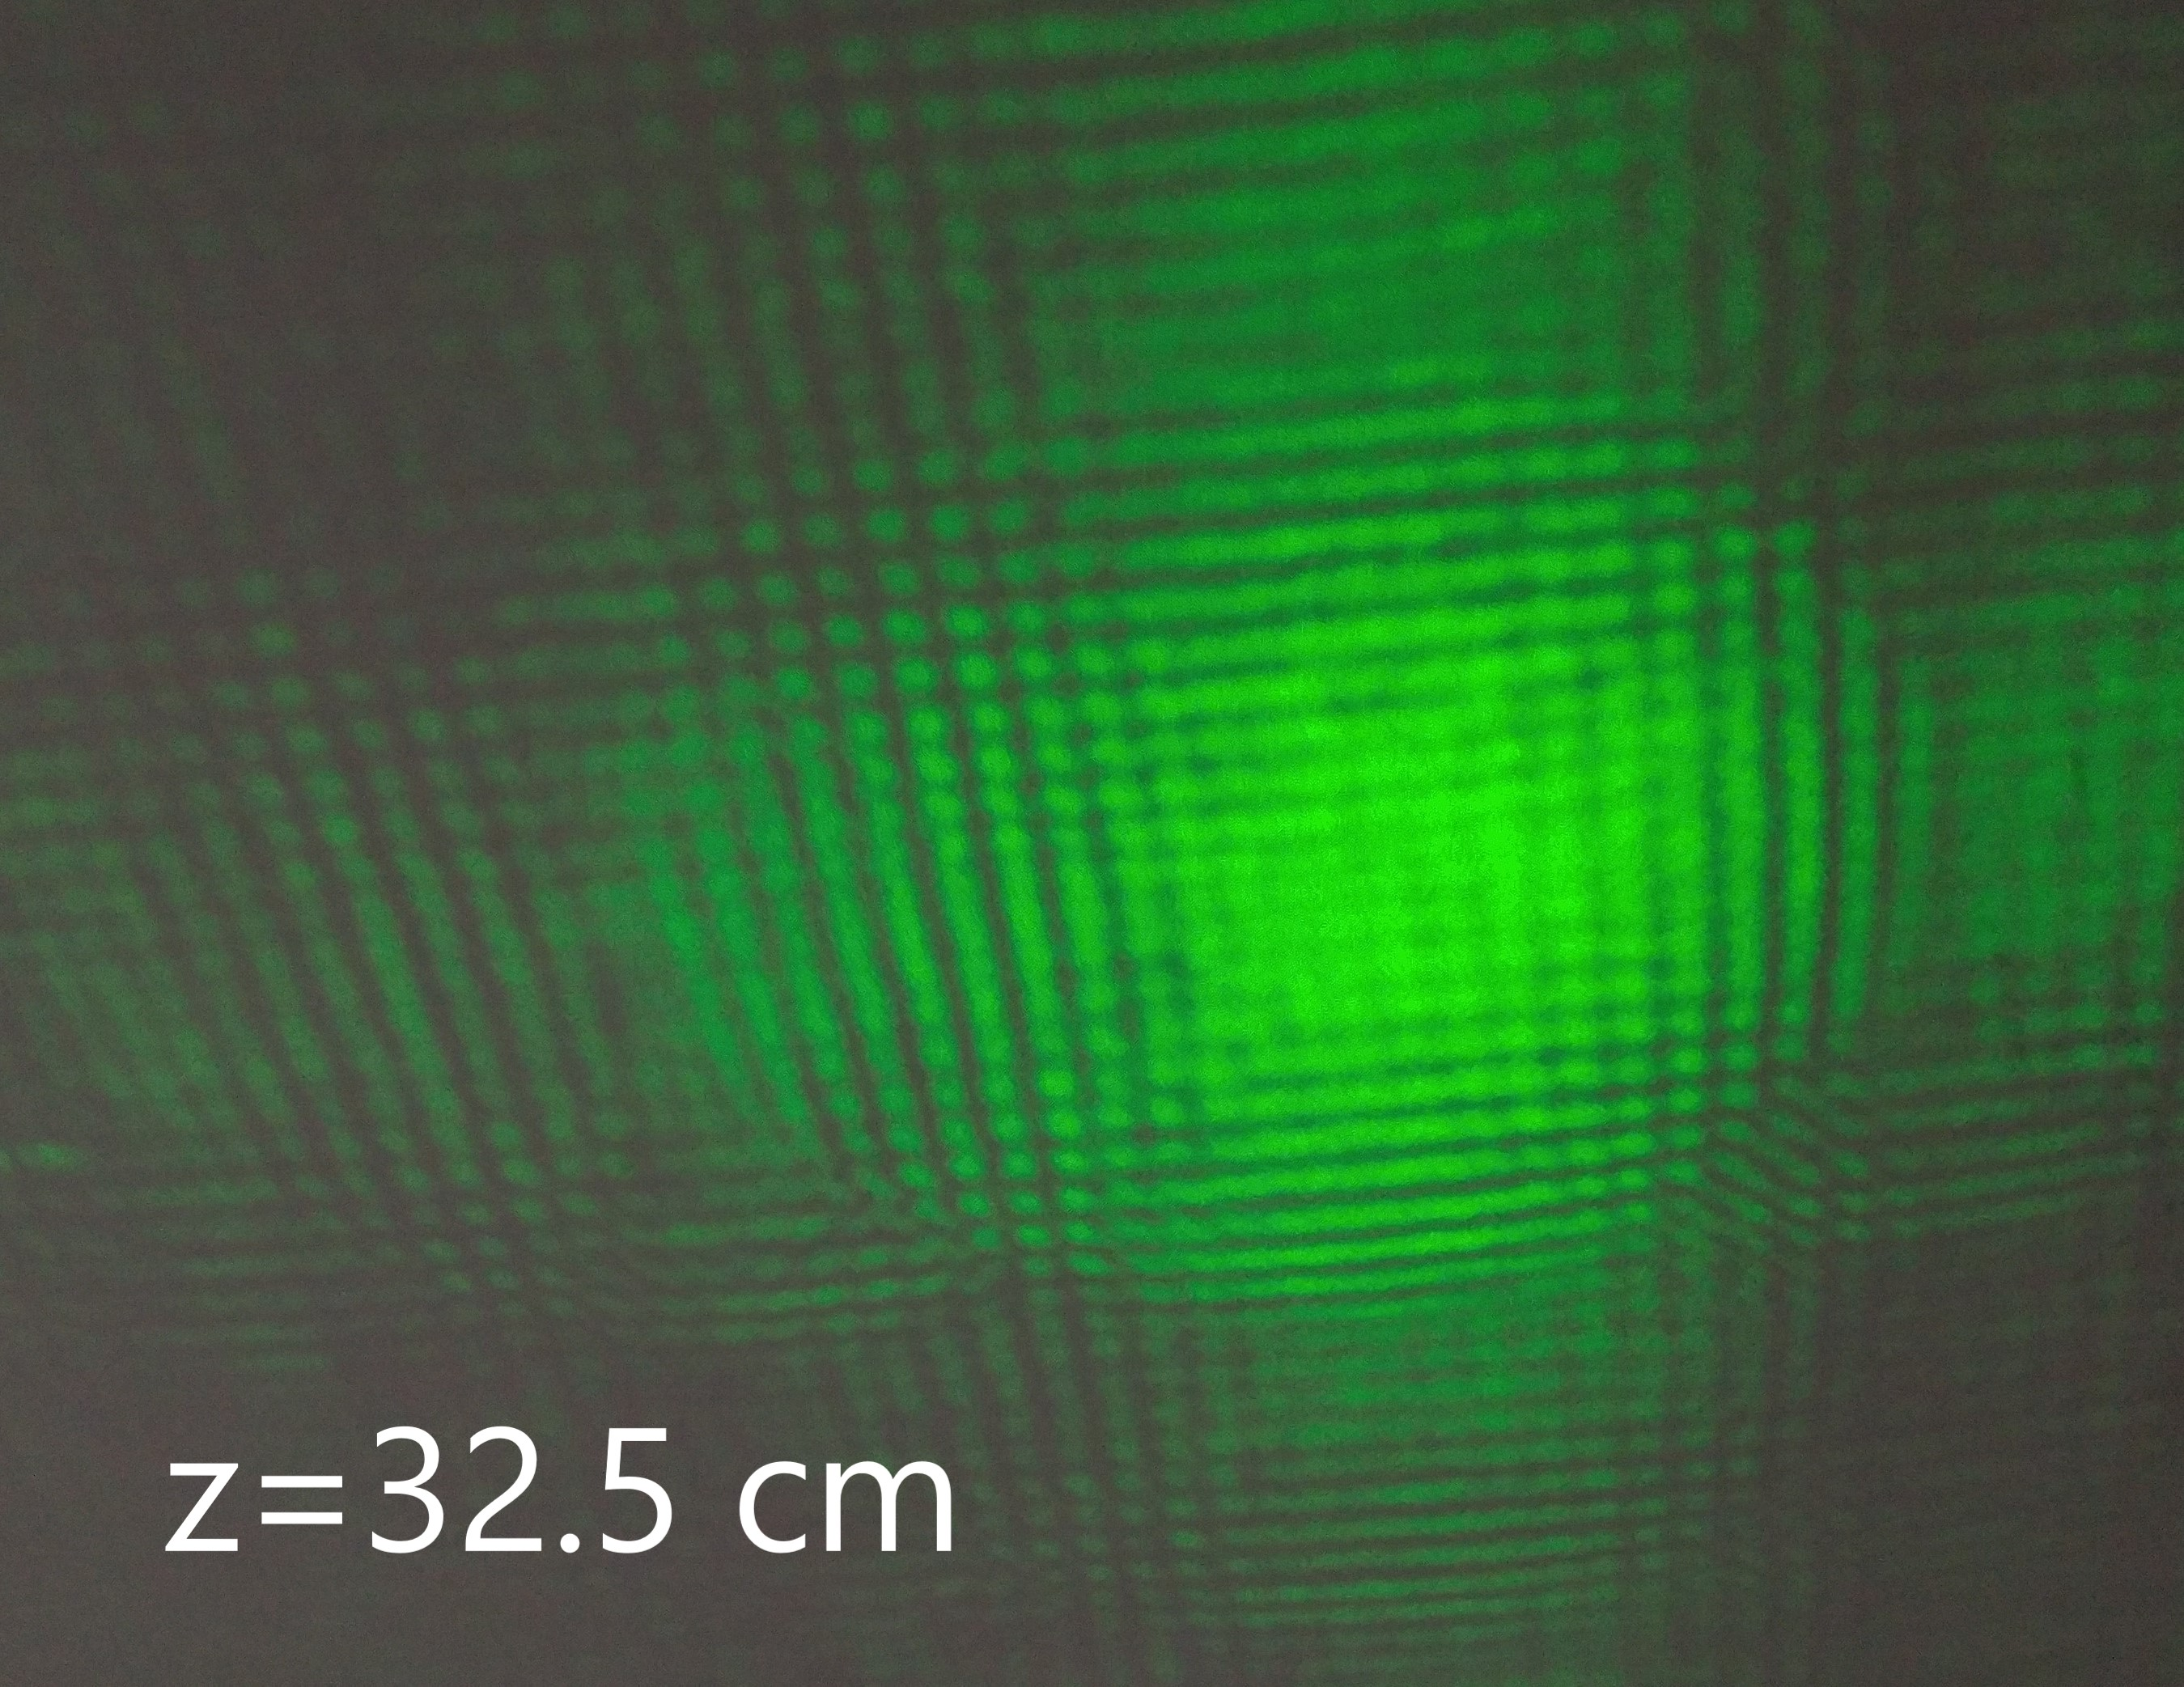
\includegraphics[width=1\linewidth]{48}
\caption{}
\label{ris:experimcoded}
\end{minipage}
\end{center}
\end{figure}  








\end{document} % конец документа
